\documentclass[12pt]{article}
\usepackage[utf8]{inputenc}
\usepackage[T1]{fontenc} % uses T1 fonts (better quality)
\usepackage{lmodern} % uses Times fonts
% \usepackage{mathptmx} % uses Times fonts
% \mathrm = un-italicize math fonts
\usepackage[dvipsnames]{xcolor}
\usepackage[margin=1in]{geometry}
\usepackage{nopageno} % no page numbers
\usepackage{graphicx}
\usepackage{pdfpages}
\usepackage{bm}
\graphicspath{ {./img/} }
\usepackage{booktabs}   % for table borders
\usepackage{amsmath}
\usepackage[makeroom]{cancel}
\usepackage{tikz}
\usetikzlibrary{shapes,arrows}

\begin{document}
 	\begin{center}
    \line(1,0){300}\\[0.25cm]
 	\Large{\bfseries ECE540: Homework \#1}\\
 	\textsc{\large David Kirby}\\
 	\textsc{\large Due: 07 September 2020}\\
 	\line(1,0){300}\\[0.75cm]
 	\end{center}

% Define block styles
% \tikzstyle{decision} = [diamond, draw, fill=blue!20,
%     text width=4.5em, text badly centered, node distance=3cm, inner sep=0pt]
\tikzstyle{block} = [rectangle, draw,
    text width=20em, text centered, rounded corners, minimum height=1em]
\tikzstyle{line} = [draw, -latex']
\tikzstyle{cloud} = [draw, ellipse,fill=red!20, node distance=3cm,
    minimum height=2em]

\begin{enumerate}
\item R2. The word \textit{protocol} is often used to describe diplomatic relations. How does Wikipedia describe diplomatic protocol?\\[1em]
Wikipedia describes diplomatic protocol as ``a rule which describes how an activity should be performed.''

\item R3. Why are standards important for protocols?\\[1em]
Standards allow different devices and protocols to communicate with each other.

\item R13. Suppose users share a 2 Mbps link. Also suppose each user transmits continuously at 1 Mbps when transmitting, but each user transmits only 20 percent of the time.
    \begin{enumerate}
        \item When circuit switching is used, how many users can be supported?\\[1em]
        Two users can be supported (each user will utilize half of the available bandwidth).
        \item For the remainder of this problem, suppose packet switching is used. Why will there be essentially no queuing delay before the link if two or fewer users transmit at the same time? Why will there be a queuing delay if three users transmit at the same time?\\[1em]
        With packet switching, each user will use 1Mbps. With a pipe of 2Mbps, two or fewer users will experience no queuing delay, but three would require 3Mbps and will result in queueing delay.
        \item Find the probability that a given user is transmitting.\\[1em]
        0.2 (given in the problem)
        \item Suppose now there are three users. Find the probability that at any given time, all three users are transmitting simultaneously. Find the fraction of time during which the queue grows.\\[1em]
        \(\binom{n}{k}
        \cdot p^{k}
        \cdot \left(1-p\right)^{n-k}
        =\cancelto{1}{\binom{3}{3}}
        \cdot 0.2^{3}
        \cdot\cancelto{1}{\left(1-0.2\right)^{3-3}}
        =0.008\)
    \end{enumerate}

\item R18. How long does it take a packet of length 1,000 bytes to propagate over a link of distance 2,500 km, propagation speed \(2.5 \cdot10^8\) m/s, and transmission rate 2 Mbps? More generally, how long does it take a packet of length \textit{L} to propagate over a link of distance \textit{d}, propagation speed \textit{s}, and transmission rate \textit{R} bps? Does this delay depend on packet length? Does this delay depend on transmission rate?\\[1em]
\( Delay_{propagation} = \frac{d}{s}
= \frac{2500\cdot10^3m}{2.5\cdot10^8m/s}
=0.01s\);\\[0.25em] more generally, \(\frac{d}{s}\);\\[0.25em] no, it does not depend on packet length;\\ no, it does not depend on transmission rate either.
\item R23. What are the five layers in the Internet protocol stack? What are the principal responsibilities of each of these layers?
\begin{center}
\begin{tikzpicture}[node distance = 2cm, auto]
    \node [block] (App) {Application Layer:\\ implements HTTP, SMTP, FTP protocols};
    \node [block, below of=App] (Trans) {Transport Layer:\\ implements TCP, UDP protocols};
    \node [block, below of=Trans] (Net) {Network Layer:\\ moves IP datagrams};
    \node [block, below of=Net] (Link) {Link Layer:\\ moves packets between nodes};
    \node [block, below of=Link] (Physical) {Physical Layer:\\ moves bits within the frame};
    \path [line] (App) -- (Trans);
    \path [line] (Trans) -- (Net);
    \path [line] (Net) -- (Link);
    \path [line] (Link) -- (Physical);
\end{tikzpicture}
\end{center}
\item P1. Design and describe an application-level protocol to be used between an automatic teller machine and a bank’s centralized computer. Your protocol should allow a user’s card and password to be verified, the account balance (which is maintained at the centralized computer) to be queried, and an account withdrawal to be made (that is, money disbursed to the user). Your protocol entities should be able to handle the all-too-common case in which there is not enough money in the account to cover the withdrawal. Specify your protocol by listing the messages exchanged and the action taken by the automatic teller machine or the bank’s centralized computer on transmission and receipt of messages. Sketch the operation of your protocol for the case of a simple withdrawal with no errors, using a diagram similar to that in Figure 1.2. Explicitly state the assumptions made by your protocol about the underlying end-to-end transport service.
    \newpage
    \begin{figure}[h!]
    \centering
    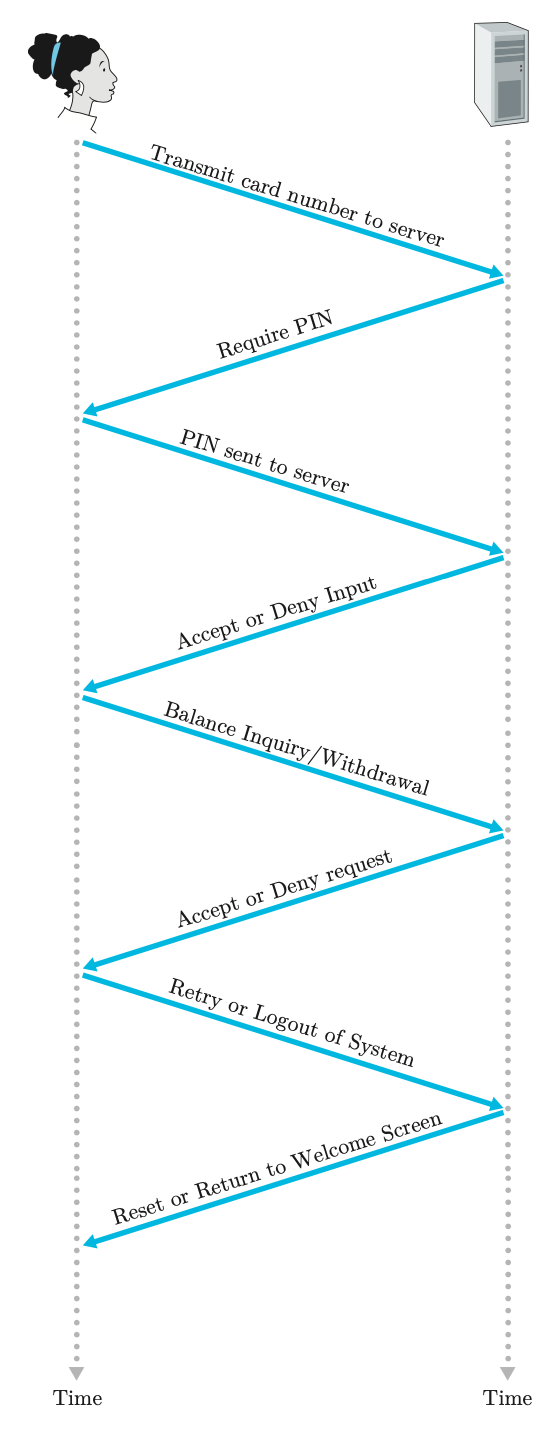
\includegraphics[width=0.45\textwidth]{Fig1.P1.png}
    % \caption{}
    % \label{fig:I2Cdemo}
    \end{figure}
Assumptions made:
\begin{itemize}
    \item secure connection
    \item congestion control
    \item reliable transport
    \item flow control
\end{itemize}

\item P4. Consider the circuit-switched network in Figure 1.13. Recall that there are 4 circuits on each link. Label the four switches A, B, C, and D, going in the clockwise direction.
    \begin{figure}[h!]
    \centering
    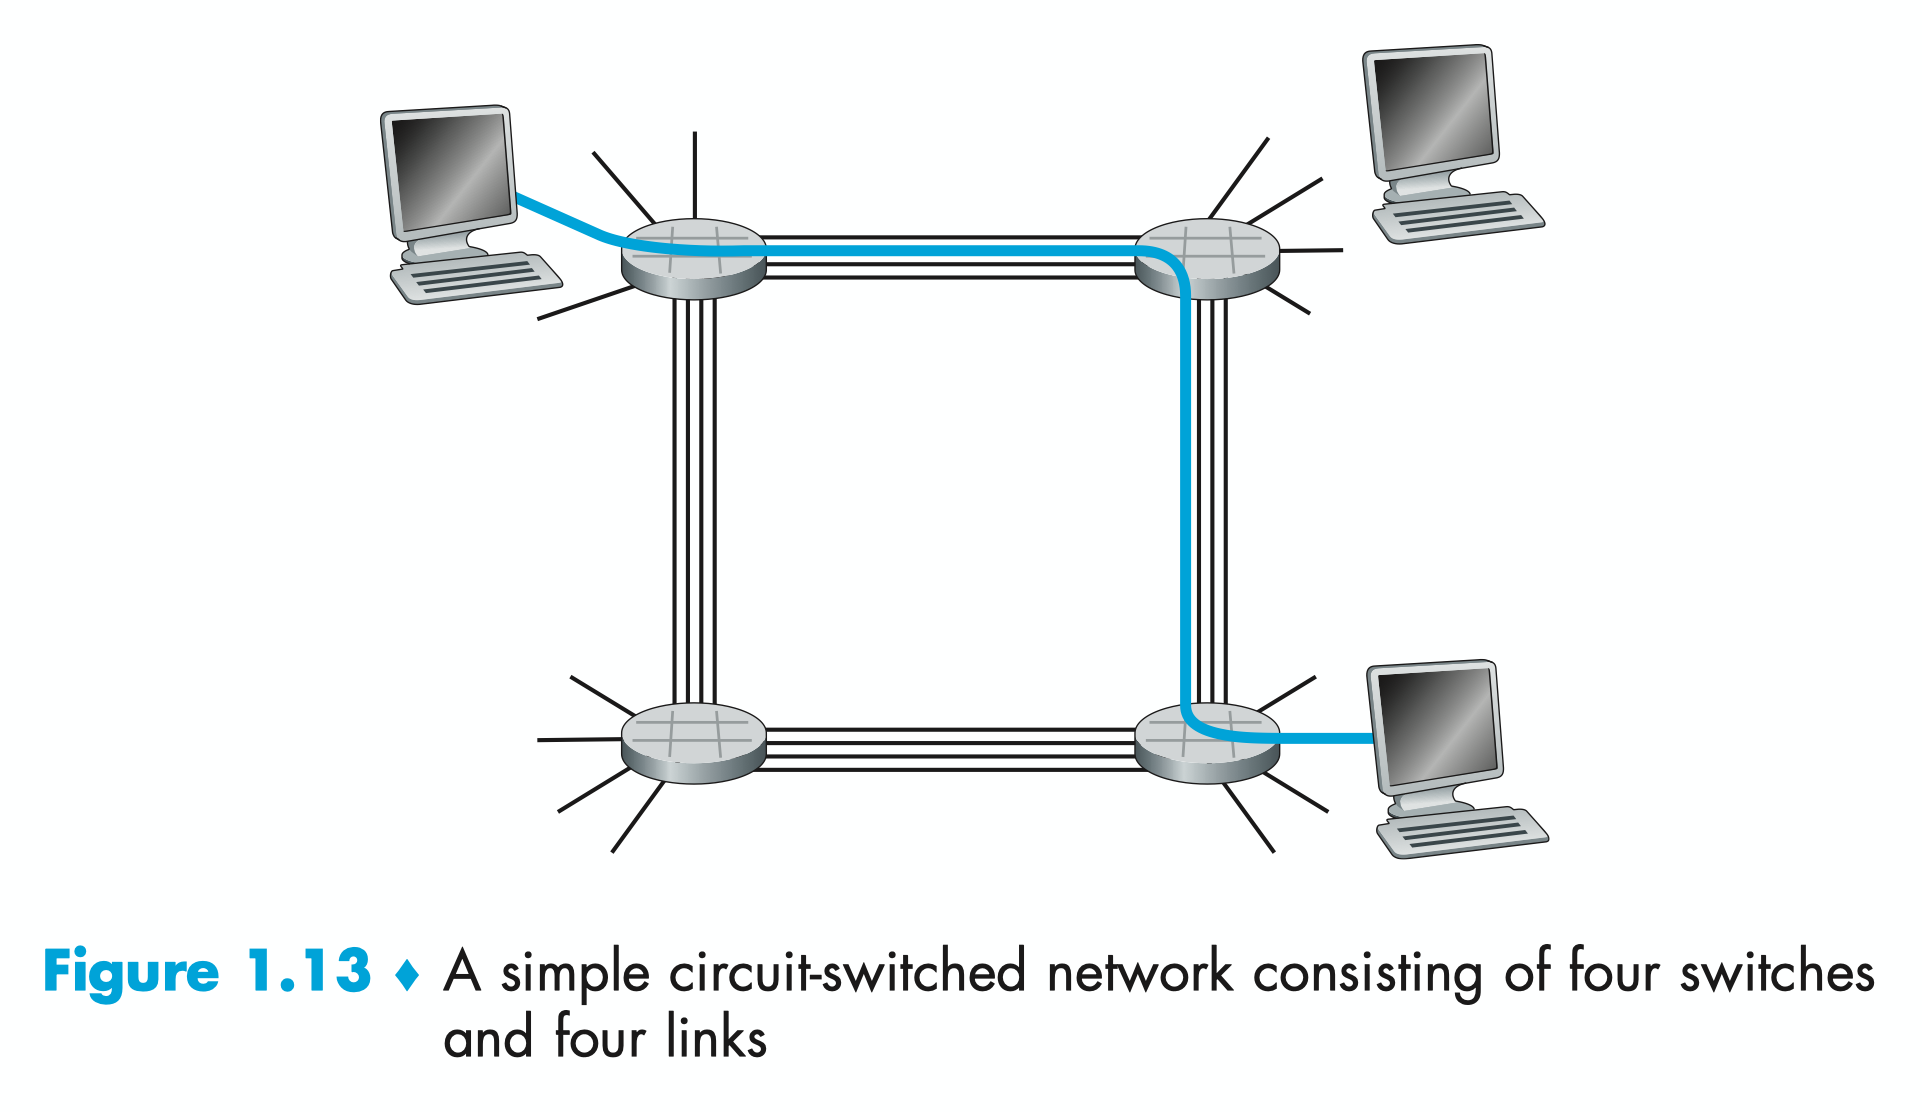
\includegraphics[width=0.88\textwidth]{Fig1.13.png}
    % \caption{}
    % \label{fig:I2Cdemo}
    \end{figure}
    \begin{enumerate}
        \item What is the maximum number of simultaneous connections that can be in progress at any one time in this network?\\[1em]
        We can have four connections between each switch for a total maximum of sixteen connections.
        \item Suppose that all connections are between switches A and C. What is the maximum number of simultaneous connections that can be in progress?\\[1em]
        Four connections in each switch, therefore a maximum of eight simultaneous connections.
        \item Suppose we want to make four connections between switches A and C, and another four connections between switches B and D. Can we route these calls through the four links to accommodate all eight connections?\\[1em]
        Yes, this is possible. We could send two through B, two through D, and alternatively send two through A while sending two through C.
    \end{enumerate}
\newpage
\item P16. Consider a router buffer preceding an outbound link. In this problem, you will use Little’s formula, a famous formula from queuing theory. Let \textit{N} denote the average number of packets in the buffer plus the packet being transmitted. Let \textit{a} denote the rate of packets arriving at the link. Let \textit{d} denote the average total delay (i.e., the queuing delay plus the transmission delay) experienced by a packet. Little’s formula is \(N  =  a \cdot d\). Suppose that on average, the buffer contains 10 packets, and the average packet queuing delay is 10 msec. The link’s transmission rate is 100 packets/sec. Using Little’s formula, what is the average packet arrival rate, assuming there is no packet loss?\\[1em]
\(N=a\cdot d\qquad
\rightarrow\qquad
a=\frac{N}{d}=\)
\resizebox{5em}{!}{\(\frac{10+1}{10ms+\frac{1}{100}}\)}
\(=550 \frac{packets}{s}\)

\item P24. Suppose you would like to urgently deliver 40 terabytes of data from Boston to Los Angeles. You have available a 100 Mbps dedicated link for data transfer. Would you prefer to transmit the data via this link or instead use FedEx overnight delivery? Explain.\\[1em]
\resizebox{10em}{!}{
\(
    \frac{40\cdot 10^{12}\ bytes \cdot 8\ bits}{100\cdot 10^6\ bps}
\)
}
\(=37.037 days\)\\[0.5em]
Over a month to transmit via this link versus overnight shipping means FedEx is the obvious choice.
\item P31. In modern packet-switched networks, including the Internet, the source host segments long, application-layer messages (for example, an image or a music file) into smaller packets and sends the packets into the network. The receiver then reassembles the packets back into the original message. We refer to this process as \textit{message segmentation}. Figure 1.27 illustrates the end-to-end transport of a message with and without message segmentation. Consider a message that is \(8 \cdot 10^6\)  bits long that is to be sent from source to destination in Figure 1.27. Suppose each link in the figure is 2 Mbps. Ignore propagation, queuing, and processing delays.
\begin{figure}[h!]
    \centering
    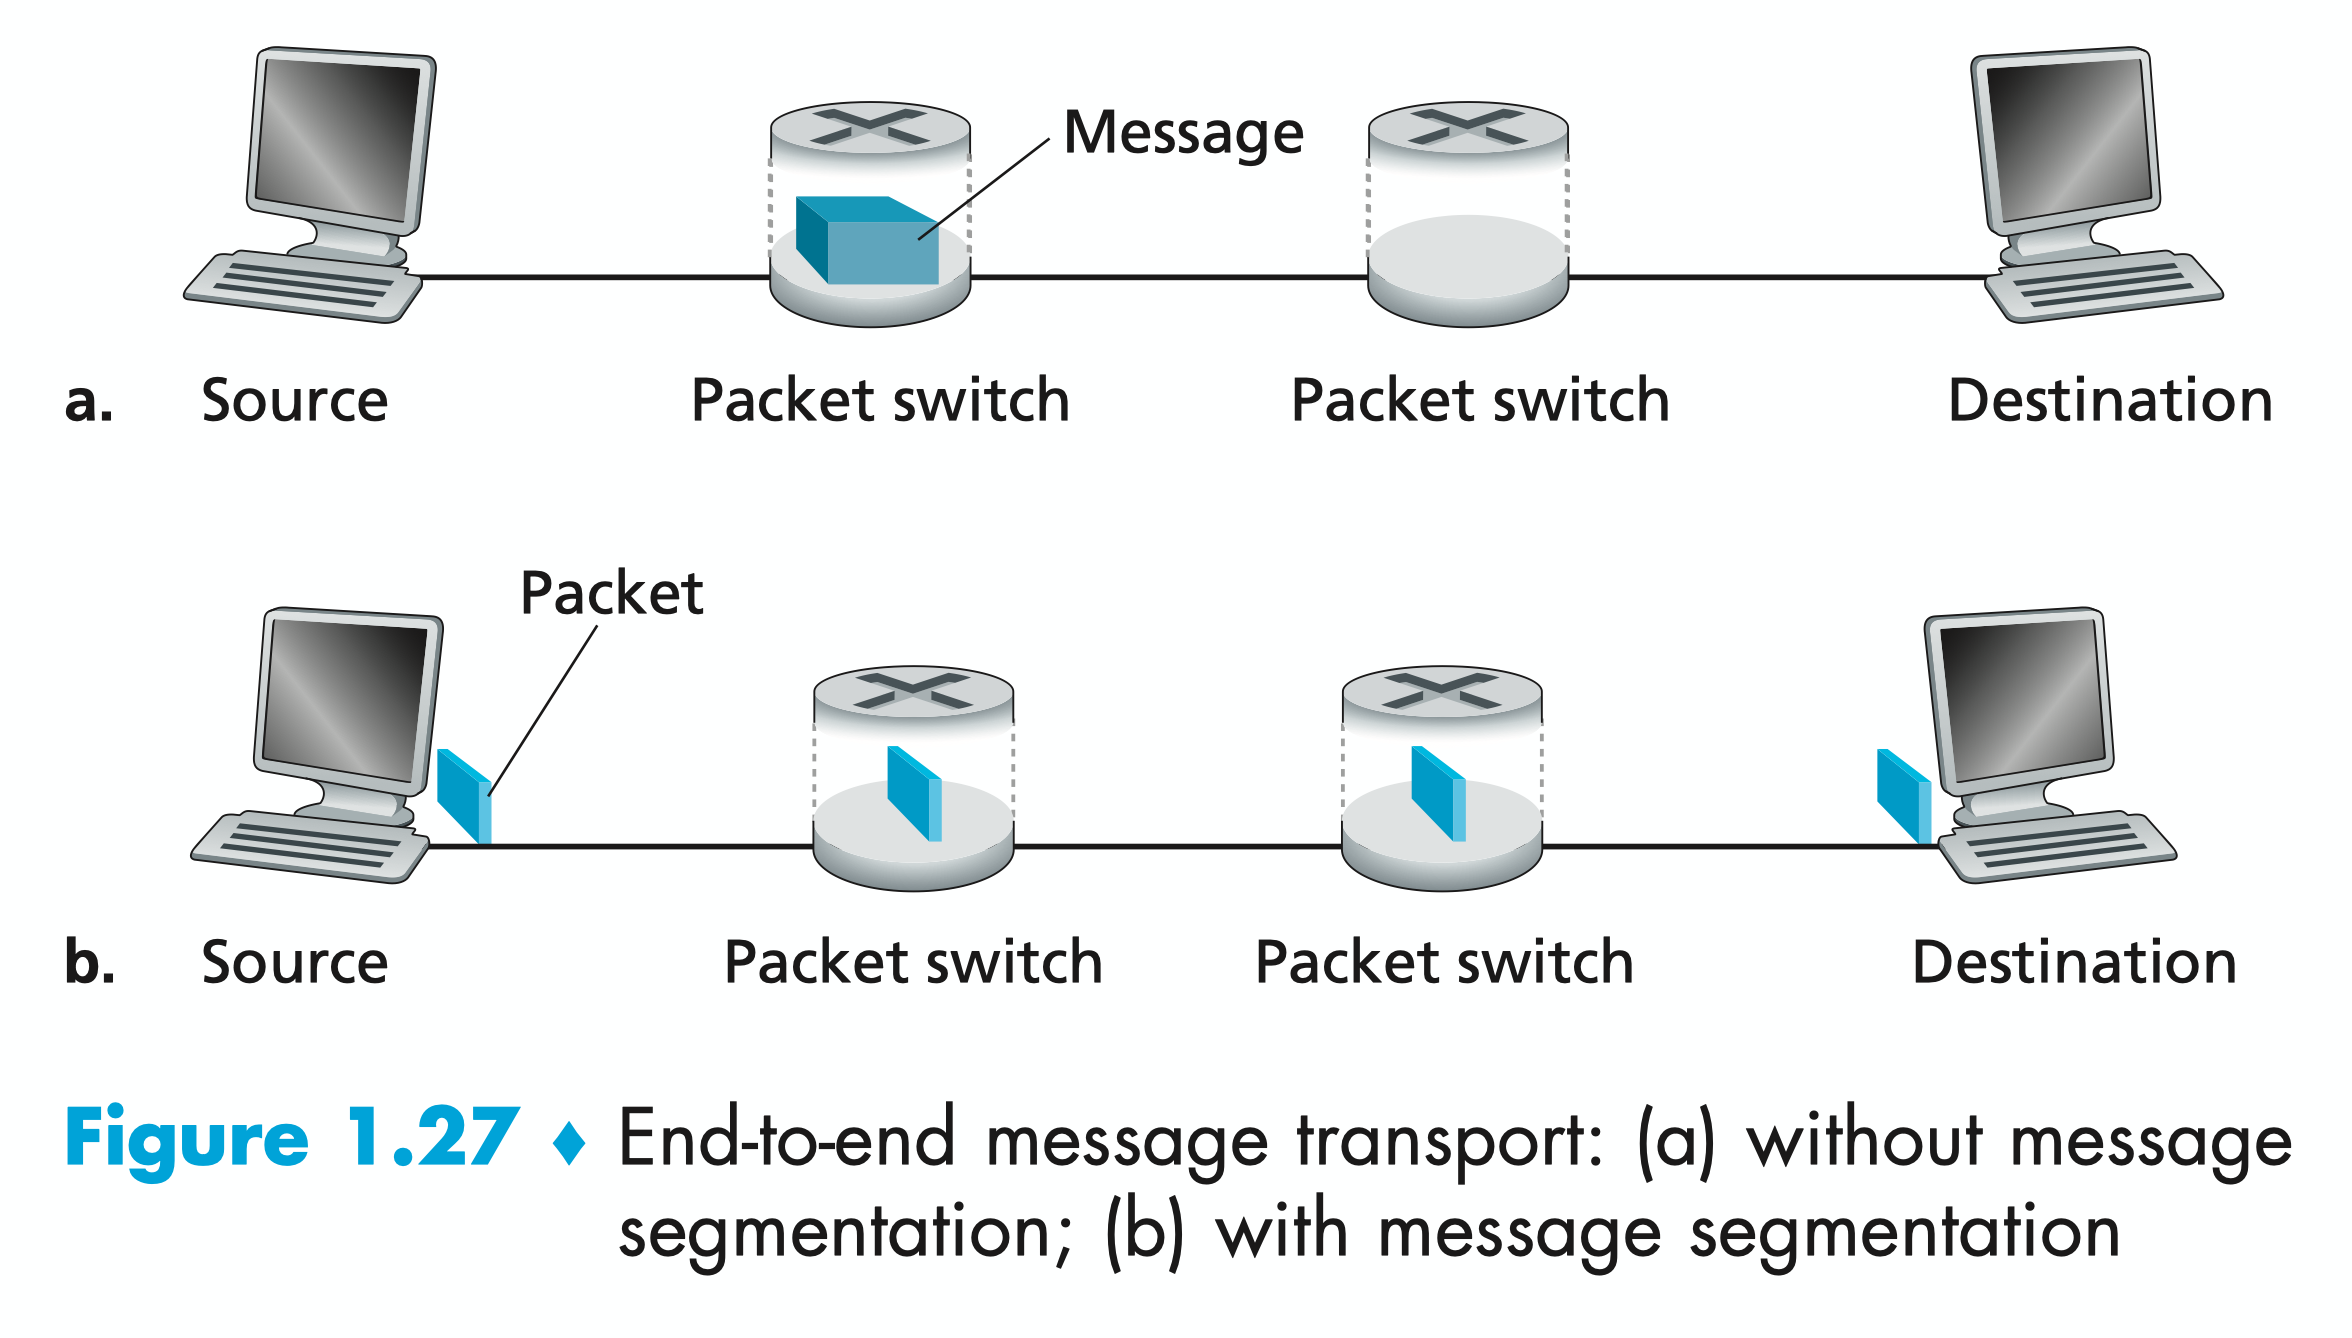
\includegraphics[width=0.78\textwidth]{Fig1.27.png}
    % \caption{}
    % \label{fig:I2Cdemo}
    \end{figure}

    \begin{enumerate}
        \item Consider sending the message from source to destination without message segmentation. How long does it take to move the message from the source host to the first packet switch? Keeping in mind that each switch uses store-and-forward packet switching, what is the total time to move the message from source host to destination host?\\[1em]
        \resizebox{5em}{!}{
        \(
            \frac{8\cdot10^6\ bits}{2\cdot10^6\ bps}
        \)}
        \(\ =4s\)\\[0.5em]
        Without message segmentation, this is 12 seconds total time.
        \item Now suppose that the message is segmented into 800 packets, with each packet being 10,000 bits long. How long does it take to move the first packet from source host to the first switch? When the first packet is being sent from the first switch to the second switch, the second packet is being sent from the source host to the first switch. At what time will the second packet be fully received at the first switch?\\[1em]
        \(
        Time_{transmission}=
        \)
        \resizebox{10em}{!}{
        \(\frac{packets}{R}
        =\frac{1\cdot10^4\ bits}{2\cdot10^6\ bps}
        \)}\(
        =0.005s
        \)\\[0.5em]
        The second packet will be fully received at the first switch at 0.01\textit{s}
        \item How long does it take to move the file from source host to destination host when message segmentation is used? Compare this result with your answer in part (a) and comment.\\[1em]
        When message segmentation is used, the time for initial packet will be 0.005\textit{s} per hop, so 0.015\textit{s}, so for 800 packets, the total time will be 4.01\textit(s); message segmentation is therefore much faster (four seconds versus twelve seconds).
        \item In addition to reducing delay, what are reasons to use message segmentation?\\[1em]
        If there is a bit error without segmentation, the entire message must be retransmitted.
        \item Discuss the drawbacks of message segmentation.\\[1em]
        Messages must be reassembled at the destination, which requires time and computational resources.
    \end{enumerate}

\end{enumerate}
\end{document}